\section{Auswertung}
\label{sec:Auswertung}

%\begin{figure}
%  \centering
%  \includegraphics{plot.pdf}
%  \caption{Plot.}
%  \label{fig:plot}
%\end{figure}
\subsection{Fourier-Analyse}
Die gemessenen Amplituden werden auf die Amplitude der ersten Oberwelle normiert. Gemessene Amplituden, sowie die Normierung 
dieser ist in \autoref{tab:amplituden} für alle drei Schwingungsformen zu sehen.
\begin{table}[!htp]
\centering
\caption{Amplituden, sowie deren Normierung auf die erste Oberwelle}
\label{tab:amplituden}
\begin{tabular}{c c c c c c c }
\toprule
& \multicolumn{2}{c}{Rechteck} &  \multicolumn{2}{c}{Sägezahn} & \multicolumn{2}{c}{Dreieck} \\
 \cmidrule(lr){2-3} 
  \cmidrule(lr){4-5}
   \cmidrule(lr){6-7}
{n} & {$U_n$ / mV} & {$\frac{U_n}{U_1}$} & {$U_n$ / mV} & {$\frac{U_n}{U_1}$} & {$U_n$ / mV} & {$\frac{U_n}{U_1}$}  \\
\midrule
1 & 2000 & 1.000 & 2160 & 1.000 & 2800  & 1.000  \\
2 & 712 & 0.356  & 1030 & 0.477 & 272 & 0.097 \\
3 & 432 & 0.216  & 656 & 0.304 & 102 & 0.036 \\
4 & 288 & 0.144  & 552 & 0.256 & 50 & 0.018 \\
5 & 216 & 0.108  & 448 & 0.207 & 28 & 0.010 \\
6 & 200 & 0.100  & 384 & 0.178 & 22 & 0.008 \\
7 & 168 & 0.084  & 312 & 0.144 &    &  \\
8 & 144 & 0.072  & 264 & 0.122 &    &  \\
9 & 112 & 0.056  & 248 & 0.115 &    &  \\
10 & 104 & 0.052 & 232 & 0.107 &    &  \\
\bottomrule
\end{tabular}
\end{table}
Die Normierungen werden doppellogarithmisch gegen die Nummer der Oberwellen aufgetragen, worüber anschließend eine lineare
Ausgleichsrechnung durchgeführt wird. Dies ist nötig um die Genauigkeit der Messung hinsichtlich des Abfalls der Oberwellenamplituden
zu überprüfen, da diese mit dem Faktor $\frac{1}{n}$ beziehungsweise $\frac{1}{n^2}$ bei der Dreieckschwinung abnehmen sollen, wie 
bereits in \autoref{sec:vorbereitung} ermittelt wurde.
Durch eine doppellogarithmische Auftragung und anschließender Bestimmung der Steigung der Ausgleichsgeraden kann diese mit dem 
theoretischen Faktor von $-1$ bei der Rechteck - und Sägezahnschwingung und $-2$ bei der Dreieckschwinung verglichen werden. 
Bei allen Schwingungsformen wird eine Ausgleichsrechnung der Form 
\begin{equation}
y = a \cdot x + b.
\end{equation} 
durchgeführt, wobei $y$ die Normierung der Amplituden  $\frac{U_n}{U_1}$ ist und  $x$ die Nummer der Oberwellen $n$.
Die Steigung $a$ der Ausgleichsgerade errechnet sich über 
\begin{equation}
\label{eqn:a}
a = \frac {\sum_{i=1}^N (x_i - \overline{x}) (y_i - \overline{y})}{\sum_{i=1}^N (x_i - \overline{x})^2}
\end{equation}
und die Konstante $b$ über
\begin{equation}
\label{eqt:b}
b = \overline{y} - a \cdot \overline{x},
\end{equation}
wobei $N$ jeweils die Gesamtanzahl der verwendeten Oberwellen ist.
Die Mittelwerte $\overline{x}$ sind mit 
\begin{equation}
\label{eqt:mittelwert}
\overline{x} = \frac {1} {N} \sum_{i=1}^N x_i
\end{equation}
zu berechnen und haben den Fehler
\begin{equation}
\label{eqt:FehlerMittelwert}
\Delta \overline{x} = \frac{1}{\sqrt{N \cdot (N-1)}} \sqrt{ \sum_{i=1}^N (x_i - \overline{x})^2}.
\end{equation}

Die aufgetragenen Werte aus \autoref{tab:amplituden}, 
sowie die Ausgleichsgerade zur Rechteckschwingung sind in \autoref{fig:graph_rechteck} zu sehen.
Bei der Reckteckschwingung, sowie bei der Sägezahnschwingung werden jeweils $N = 10$ Amplitudenverhältnisse eingebracht.
Bei der Rechteckschwingung ist außerdem zu Beachten, dass, wie in \autoref{sec:vorbereitung} festgestellt, nur die 
ungeraden Koeffizienten einwirken, sodass hier die ersten zehn Amplitudenverhältnisse ungerader Oberwellennummer aufgetragen
werden.
Die Steigung der linearen Ausgleichsgerade zur Rechteckschwingung beträgt nach Gleichung \eqref{eqn:a}
\\ \\
\centerline{$a = ( -1.002 \pm 0.021 ) $.}
\\ \\
\begin{figure}
  \centering
  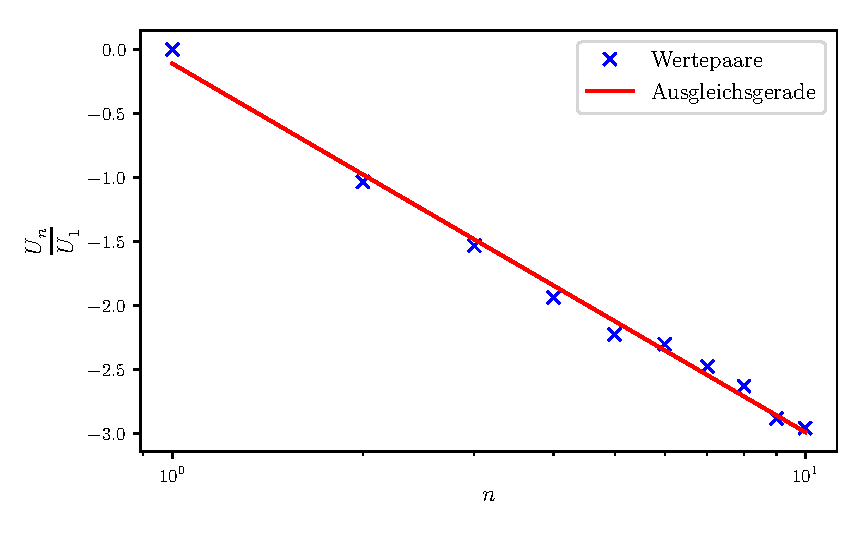
\includegraphics{build/rechteck.pdf}
  \caption{Normierungen der Amplituden der Rechteckschwingung doppellogarithmisch gegen die Nummer der Oberwellen aufgetragen mit zugehöriger Ausgleichsgerade.}
  \label{fig:graph_rechteck}
\end{figure}
Bei der Sägezahnschwingung sind die entsprechenden, aufgetragenen Werte aus \autoref{tab:amplituden}, sowie die zugehörige Ausgleichsgerade
in \autoref{fig:graph_saegezahn} zu sehen. 
Die Steigung der Ausgleichsgerade beträgt mit Gleichung \eqref{eqn:a}
\\ \\ 
\centerline{$ a = (- 0.966 \pm 0.021)$.}
\\ \\
\begin{figure}
  \centering
  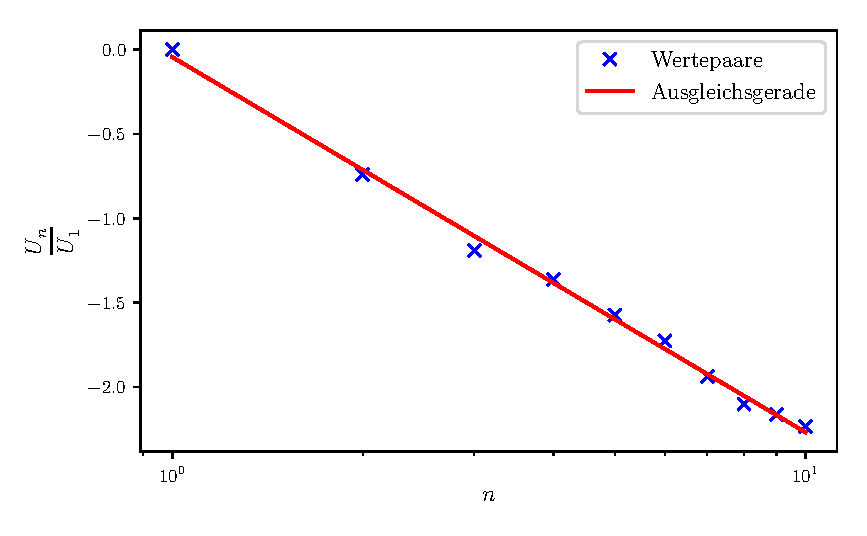
\includegraphics{build/saegezahn.pdf}
  \caption{Normierungen der Amplituden der Sägezahnschwinung doppellogarithmisch gegen die Nummer der Oberwellen aufgetragen mit zugehöriger Ausgleichsgerade.}
  \label{fig:graph_saegezahn}
\end{figure}
Statt einer Anzahl von $N = 10$ Oberwellen, liegen hier lediglich $N = 6$ Oberwellen vor (siehe \autoref{sec:Diskussion}),
wobei auch hier wieder nur Oberwellen ungerader Nummer einwirken.
Die Werte werden entsprechend wieder aus \autoref{tab:amplituden} entnommen und doppellogarithmisch gegen die Anzahl der 
Oberwellen aufgetragen, worüber wieder eine Ausgleichsgerade gebildet wird. Dies ist in \autoref{fig:graph_dreieck} zu sehen.
Die Steigung der Ausgleichsgerade beträgt 
\\ \\
\centerline{$a = ( -2.041 \pm 0.037 )$.}
\\ \\
\begin{figure}
  \centering
  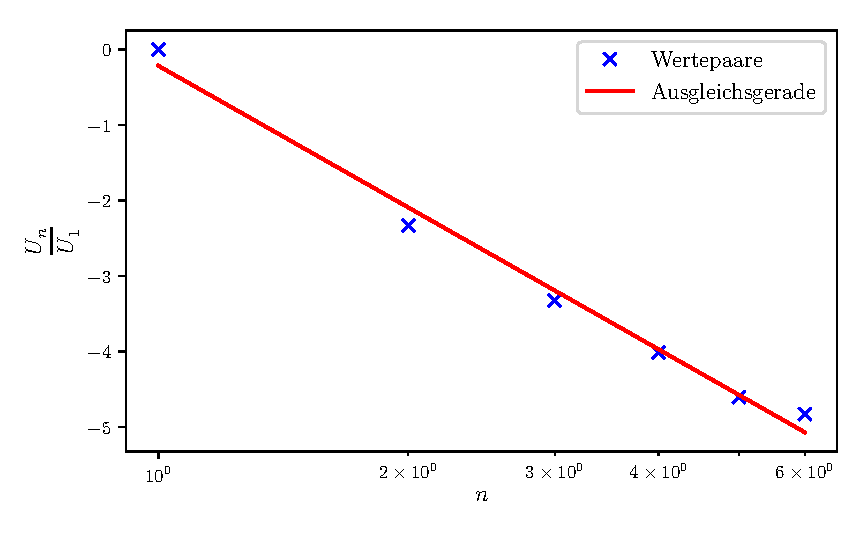
\includegraphics{build/dreieck.pdf}
  \caption{Normierungen der Amplituden der Dreieckschwinung doppellogarithmisch gegen die Nummer der Oberwellen aufgetragen mit zugehöriger Ausgleichsgerade.}
  \label{fig:graph_dreieck}
\end{figure}
\newpage
\subsection{Fourier-Synthese}
Die zur Fouriersynthese verwendeten Amplituden sind in \autoref{tab:eingestellt} zu sehen. 
\begin{table}[!htp]
\centering
\caption{Eingestellte Amplituden zur Fouriersynthese zu den drei Schwingungsformen.}
\label{tab:eingestellt}
\begin{tabular}{c c c}
\toprule
 & \multicolumn{2}{c}{Eingestellte Amplituden $U$ / mV } \\
 \cmidrule(lr){2-3}
{Nummer der Oberwelle} & {Reckteck und Sägezahn} & {Dreieck} \\
\midrule
1 & 709.00 & 712.0\\
2 & 354.50 & 178.0\\
3 & 236.30 & 79.1\\
4 & 177.25 & 44.5\\
5 & 141.80 & \\
6 & 118.16 & \\
7 & 101.28 & \\
8 & 88.625 & \\
9 & 78.80  & \\
10 & 70.90 & \\
\bottomrule
\end{tabular}
\end{table}
Bei der Synthese der Rechteckschwingung werden die entsprechenden Werte aus \autoref{tab:eingestellt} entnommen, wobei in die 
Rechteckschwingung nur Oberwellen mit ungerader Nummer einwirken; Oberwellen mit gerader Nummer sind bei der Rechteckschwingung
zu vernachlässigen. Die synthetisierte Funktion ist in \autoref{fig:synth_rechteck} dargstellt. Diese lässt sich gut als 
Darstellung einer Rechteckfunktion identifizieren, wobei an den Extrema der Rechteckfunktion weitere kleinere Minima und Maxima
zu erkennen sind. Des Weiteren treten diese kleineren Minima und Maxima nicht konstant auf einer Höhe auf, sondern sind 
in ihrer Höhe an den Maxima der Rechteckfunktion leicht fallend und an den Minima der Rechteckfunktion leicht steigend. 
\begin{figure} 
  \centering
  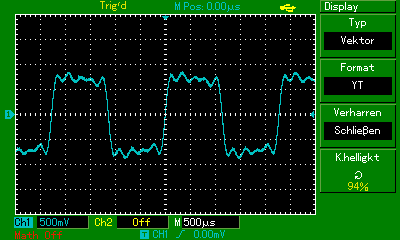
\includegraphics{content/MAP002.png}
  \caption{Synthetisierte Rechteckschwingung.}
  \label{fig:synth_rechteck}
\end{figure}

Bei der Synthese der Sägezahnschwingung werden dieselben Koeffizienten wie bei der Synthese der Rechteckschwingung verwendet, da
die Koeffizienten beider Schwingungsformen mit dem selben Faktor $\frac{1}{n}$ abfallen. Hier wirken allerdings alle 
entsprechende Werte aus \autoref{tab:eingestellt} ein. Die synthetisierte Sägezahnfunktion 
ist in \autoref{fig:synth_saegezahn} zu sehen. Auch die Sägezahnschwingung ist eindeutig zu erkennen. An der linken Flanke 
der Amplituden sind deutliche Nebenschwingungen auszumachen, welche teilweise sehr flach ausfallen, aber auch steilere 
Nebenamplituden auftreten. Die rechte Flanke, ist sehr steil fallend, aber dennoch Ungenauigkeiten in Form von kleineren
Nebenschwingungen unterworfen.

\begin{figure}
  \centering
  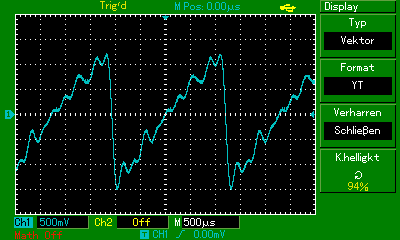
\includegraphics{content/MAP001.png}
  \caption{Synthetisierte Sägezahnschwingung.}
  \label{fig:synth_saegezahn}
\end{figure}

Zur Synthese der Dreieckschwingung werden die entsprechenden Amplituden (von Oberwellen ungerader Nummer) aus \autoref{tab:eingestellt} verwendet.
Die so synthetisierte Dreieckschwingung ist in \autoref{fig:synth_dreieck} zu sehen. Die dargstellte Schwingung ist als 
Dreieckschwingung auszumachen. An der linken Flanke tritt eine Nebenamplitude auf, welche den Eindruck eines Knicks in der 
Flanke vermittelt. Die rechte Flanke ist von solchen Ungenauigkeiten nicht betroffen, scheint aber dennoch nicht gerade zu
verlaufen, sondern einen leicht kurvenförmigen Verlauf zu nehmen.  

\begin{figure}
  \centering
  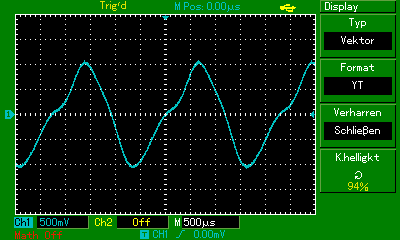
\includegraphics{content/MAP003.png}
  \caption{Synthetisierte Dreieckschwingung.}
  \label{fig:synth_dreieck}
\end{figure}